%%
% 引言或背景
% 引言是论文正文的开端,应包括毕业论文选题的背景、目的和意义;对国内外研究现状和相关领域中已有的研究成果的简要评述;介绍本项研究工作研究设想、研究方法或实验设计、理论依据或实验基础;涉及范围和预期结果等。要求言简意赅,注意不要与摘要雷同或成为摘要的注解。
% modifier: 黄俊杰(huangjj27, 349373001dc@gmail.com)
% update date: 2017-04-15
%%

\chapter{引言}
\label{cha:introduction}
\section{选题背景与意义}
\label{sec:background}
让机器节省甚至替代人力一直是科技发展的大方向。自动驾驶汽车,一种通过传感器和电脑实现无人驾驶的智能汽车,则是近些年来越来越受到关注的一个研究热点。如果自动驾驶技术能在生活中得到广泛应用,那么人们的生活质量将大幅提高。举两个很贴近校园生活的例子:很多学校都有校内接送学生的电动车,它的时间和线路相对固定,驾驶巴士的司机常年做着重复劳动,十分枯燥;很多同学喜欢叫外卖,因此无数的递送员每天奔波于商家和宿舍之间,还经常因为无法按时送达被投诉。但假如能应用成熟的自动驾驶技术,这样的情况将得到极大改善。不仅如此,在国家快速现代化发展的大环境下,自动驾驶还可以缓解城市交通拥堵、交通事故发生频繁等问题。所以,自动驾驶技术的发展对于国家和社会具有重要意义。

虽然自动驾驶技术距离广泛应用还有一定的距离,但相关研究工作已经在国内外各大企业和高校如火如荼地展开。为了方便区分和定义自动驾驶的程度,国际自动机工程师学会(SAE)提出了一套分级标准,将自动驾驶分为了L0到L5六个等级(如图1-1)。其中L0和L1实现自动化的程度非常低,需要人类驾驶员执行几乎所有操作。而到了L2,控制方向和加减速的操作就可以由汽车自己完成,驾驶员需要监视,准备随时接管以完成其他操作。到了L3,驾驶员已经可以解放手脚了,但仍需保持注意力集中。而L4和L5则已经无需驾驶员的控制,完全由汽车自己掌握全部操作,只是L4对道路环境有特殊要求。目前很多汽车制造商的技术都达到了L2级别,比如Tesla的Autopilot 2.0和Volvo的S60。谷歌测试中的无人车处在L3的阶段。而硅谷一家2016年成立的公司Nuro声称他们的配送车可以不用人类驾驶员,也就是至少达到了L4的水平。
\begin{figure}[h]
	\centering
	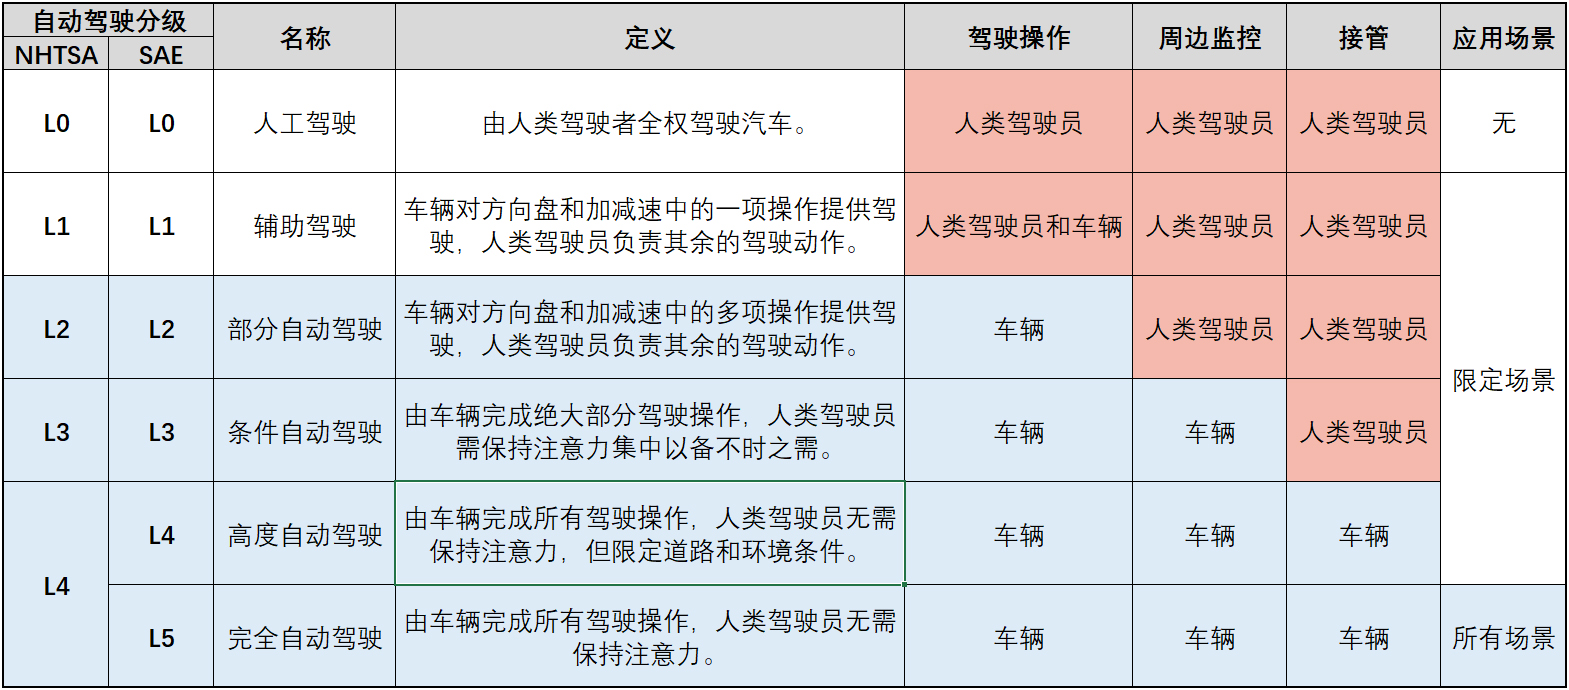
\includegraphics[width=0.5\textwidth]{image/自动驾驶等级.jpg}
	\caption{SAE提出的自动驾驶等级}
 	\label{fig:1-1}
\end{figure}


自动驾驶中的一大难点是环境感知,即采用什么样的传感器,以及如何将传感器采集的环境数据转化为机器可以理解的数据。对于这个问题,不同的实验室有不同的解决方案。Tesla使用的是视觉摄像头。由于视觉摄像头成本低廉,且图像检测算法已经较为成熟,所以纯视觉方法应用更为广泛。但是视觉摄像头,无论单目还是多目,都很难捕捉到准确的三维信息,因为它们很容易受到环境中光线变化、障碍物遮挡等的影响。谷歌旗下的Waymo和百度的Apollo则更多使用激光雷达。激光雷达的优点在于稳定性高,对空间感知能力强。然而它的成本高昂,且基于它采集的三维数据的算法复杂度较高,所以如何将其很好地应用还有待进一步研究。

\section{问题描述}
\label{sec:problem_description}
自动驾驶场景下的三维物体追踪,主要目标是:基于激光雷达在实际道路场景采集的三维点云数据(kitti数据集),追踪其中的多辆汽车,用三维的立方体框将它们在点云中准确地标识出来。由于数据集由一段一段连续的点云流构成,帧与帧之间不存在剧烈的变化,所以相邻帧之间的特征图具有一定的共性。如果我们能对点云流的这一特点加以利用,则将进一步提升最终的效果。

\section{本文的工作}
\label{sec:key_work}
针对上文提到的主要目标和优化方向,本项目融合了两种开源框架。其中,Voxelnet中的特征学习(feature learning)是框架的主要部分,而Detect to Track(下文简称D&T)中的相关层(correlation layer)则可以很好地发掘相邻帧之间特征的相似性。为了适配相关层的输入和输出,我们对点云读取方式和损失函数计算方式也做出了相应的调整。总结本文具体的创新和贡献如下:
\begin{itemize}
	\item 采用合并相邻两帧的方式读取点云数据。
	\item 采用Voxelnet学习特征,同时用D&T的相关层发掘相邻帧的相似性。
	\item 在损失函数中加入相关损失(correlation loss)。
\end{itemize}

\section{论文结构与章节安排}
\label{sec:arrangement}
本文共分为五章,各章节内容安排如下:

第一章引言。

第二章综述。

第三章方法、原理和框架。

第四章实验和结果。

第五章总结与展望。

